%! Author = sujal
%! Date = 9/10/24

% Preamble
%! suppress = FileNotFound
\documentclass[11pt]{ipu-ai}
\doctitle{Artificial Intelligence Lab (ARI251)}

% Packages
\usepackage{amsmath}
\usepackage{amssymb}
\usepackage[T1]{fontenc}
\usepackage[
    pdftitle={AI Lab Practical File},
    pdfsubject={AI Lab Practical File},
    pdfauthor={Sujal Singh},
    pdfdisplaydoctitle,
    hidelinks,
]{hyperref}
\usepackage{tabularray}
\usepackage{tikz}
\usepackage[indLines]{algpseudocodex}

% Document
\begin{document}
    \maketitle
    \pagenumbering{gobble}
\pagestyle{empty}
\begin{center}
    \textbf{\huge Index} \\[20pt]
    \begin{tblr}{rows={50pt},colspec={|Q[m,c]|Q[12,m]|Q[3,c]|},hlines,vlines,
        cell{2-Z}{1} = {cmd=\textbf{\the\numexpr\arabic{rownum}-1}.},
        cell{1}{2}={c}}
        \textbf{No.} & \textbf{Question} & \textbf{Remarks} \\
        &%
        Water Jug Problem
        & \\
        &%
        8 -- Tile Problem
        & \\
        &%
        Breadth First Search
        & \\
        &%
        Depth First Search
        & \\
        &%
        Graph coloring problem
        & \\
        &%
        AO* Search
        & \\
        &%
        Performing operations on array using NumPy.
        & \\
        &%
        Using pandas in python, create data frames using the same.
        & \\
    \end{tblr}
\end{center}
    % ---------------------------------------------------------------------------------------------------------------- %

    %------------------------------------------------------------------------------------------------------------------%
    %------------------------------------------------------------------------------------------------------------------%
    \experiment{1}%
    {Given two jugs with capacities 4 liters and 3 liters respectively, measure exactly 1 liter in the
    second jug, by only performing the following operations: fill either jug to full capacity, empty either jug or
    transfer water from one jug to another until either first jug is empty or the second jug is full (or vice versa).
    Find the sequence of operations that reaches the target state with the minimum amount of moves.}%
    {Given an initial and target state and the capacity of both the jugs, the \detokenize{possible_moves} function
    produces next possible states which are then appended to a queue if not already visited, each node in the queue is
    then visited (FIFO) until the current state becomes the target state or there are no possible moves left.}\\%
%    \begin{tabularsection}{Algorithm}
%        \begin{algorithmic}[1]
%            \State Start
%            \State queue $ \leftarrow \{ \text{INITIAL} \}$
%            \State visited $ \leftarrow \{\}$
%            \While{queue $ \neq \emptyset$}
%                \State \textbf{POPLEFT} from queue $\rightarrow$ current
%                \If{current $=$ TARGET}
%                    \State \Return PATH
%                \EndIf
%                \State visited.append(current)
%            \EndWhile
%            \State Stop
%        \end{algorithmic}
%    \end{tabularsection}
    \begin{code}
        {Program}{python}
from collections import deque

INITIAL, TARGET,J1_CAPACITY, J2_CAPACITY = (0, 0), (0, 1), 4, 3

def possible_moves(current_state):
    moves = {current_state}
    a, b = current_state
    # Empty
    moves.add((0, b))
    moves.add((a, 0))
    # Fill
    moves.add((J1_CAPACITY, b))
    moves.add((a, J2_CAPACITY))
    # Transfer
    moves.add((a - (transfer := min(a, J2_CAPACITY - b)), b + transfer))
    moves.add((a + (transfer := min(b, J1_CAPACITY - a)), b - transfer))
    moves.remove(current_state)
    return moves

def search(initial_state, target_state):
    queue = deque([(initial_state, [])])
    visited = set()

    while queue:
        current, path = queue.popleft()
        if current == target_state:
            return path + [current]
        visited.add(current)

        for child in possible_moves(current):
            if child not in visited:
                queue.append((child, path + [current]))
    return []

result = search(INITIAL, TARGET)
print(f"Moves: {len(result) - 1 if result else 'Unreachable Target'}\nPath: ", end="")
print(*result, sep=" -> ")
    \end{code}%
    \begin{code}
        {Output}{text}
Moves: 4
Path: (0, 0) -> (4, 0) -> (1, 3) -> (1, 0) -> (0, 1)
    \end{code}
    \newpage%

    % ---------------------------------------------------------------------------------------------------------------- %
    % ---------------------------------------------------------------------------------------------------------------- %

    \experiment{2}{8 Tile Problem.}%
    {Given an intial and target state, the program will perform A* search on the search space with the misplaced tiles
    heuristic function.}%

%    \begin{tabularsection}{Algorithm}
%        \begin{algorithmic}[1]
%            \State Start
%            \State{\textbf{print} ``Hello, World!''}
%            \State Stop
%        \end{algorithmic}
%    \end{tabularsection}%

    \begin{code}
        {Program}{python}
from copy import deepcopy
from heapq import heappush, heappop

SIZE = 3
INITIAL = [
    [1, 2, 3],
    [8, 0, 4],
    [7, 6, 5]]
TARGET = [
    [2, 8, 1],
    [0, 4, 3],
    [7, 6, 5]]
BLANK_POS = [1, 1]
ALLOWED_MOVES = ((1, 0), (-1, 0), (0, 1), (0, -1))


def heuristic(state):
    # Increases cost for every misplaced tile.
    h = 0
    for x in range(SIZE):
        for y in range(SIZE):
            if state[x][y] != TARGET[x][y]:
                h += 1
    return h


def possible_moves(state, blank_pos):
    x, y = blank_pos
    moves = []
    for i, j in ALLOWED_MOVES:
        p, q = x + i, y + j
        if not ((0 <= p <= 2) and (0 <= q <= 2)):
            continue
        next_state = deepcopy(state)
        next_state[x][y], next_state[p][q] = next_state[p][q], next_state[x][y]
        moves.append((next_state, (p, q)))
    return moves


def search():
    pq = []
    visited = set()
    heappush(pq, (heuristic(INITIAL), 0, INITIAL, BLANK_POS))

    while pq:
        h, g, current, current_blank_pos = heappop(pq)
        print(current)
        if current == TARGET:
            return
        visited.add(tuple(map(tuple, current)))

        for next_state, next_blank_pos in possible_moves(current, current_blank_pos):
            if tuple(map(tuple, next_state)) in visited:
                continue
            new_g = g + 1
            new_h = new_g + heuristic(next_state)
            heappush(pq, (new_h, new_g, next_state, next_blank_pos))


search()
    \end{code}%
    \begin{code}
        {Output}{text}
[[1, 2, 3], [8, 0, 4], [7, 6, 5]]
[[1, 2, 3], [0, 8, 4], [7, 6, 5]]
[[1, 2, 3], [8, 4, 0], [7, 6, 5]]
[[1, 2, 0], [8, 4, 3], [7, 6, 5]]
[[1, 0, 3], [8, 2, 4], [7, 6, 5]]
[[1, 0, 2], [8, 4, 3], [7, 6, 5]]
[[1, 2, 3], [8, 6, 4], [7, 0, 5]]
[[0, 1, 3], [8, 2, 4], [7, 6, 5]]
[[0, 2, 3], [1, 8, 4], [7, 6, 5]]
[[1, 2, 3], [8, 4, 5], [7, 6, 0]]
[[1, 3, 0], [8, 2, 4], [7, 6, 5]]
[[2, 0, 3], [1, 8, 4], [7, 6, 5]]
[[8, 1, 3], [0, 2, 4], [7, 6, 5]]
[[0, 1, 2], [8, 4, 3], [7, 6, 5]]
[[2, 8, 3], [1, 0, 4], [7, 6, 5]]
[[2, 8, 3], [0, 1, 4], [7, 6, 5]]
[[2, 8, 3], [1, 4, 0], [7, 6, 5]]
[[8, 1, 2], [0, 4, 3], [7, 6, 5]]
[[2, 8, 0], [1, 4, 3], [7, 6, 5]]
[[1, 2, 3], [7, 8, 4], [0, 6, 5]]
[[1, 3, 4], [8, 2, 0], [7, 6, 5]]
[[1, 4, 2], [8, 0, 3], [7, 6, 5]]
[[2, 3, 0], [1, 8, 4], [7, 6, 5]]
[[1, 4, 2], [0, 8, 3], [7, 6, 5]]
[[1, 2, 3], [8, 6, 4], [0, 7, 5]]
[[1, 2, 3], [8, 6, 4], [7, 5, 0]]
[[1, 2, 3], [0, 6, 4], [8, 7, 5]]
[[1, 2, 3], [8, 4, 5], [7, 0, 6]]
[[1, 3, 4], [8, 0, 2], [7, 6, 5]]
[[8, 1, 3], [2, 0, 4], [7, 6, 5]]
[[1, 3, 4], [0, 8, 2], [7, 6, 5]]
[[2, 3, 4], [1, 8, 0], [7, 6, 5]]
[[2, 8, 3], [1, 6, 4], [7, 0, 5]]
[[8, 1, 3], [2, 4, 0], [7, 6, 5]]
[[2, 8, 3], [1, 4, 5], [7, 6, 0]]
[[8, 1, 0], [2, 4, 3], [7, 6, 5]]
[[2, 0, 8], [1, 4, 3], [7, 6, 5]]
[[8, 0, 1], [2, 4, 3], [7, 6, 5]]
[[0, 8, 1], [2, 4, 3], [7, 6, 5]]
[[2, 8, 1], [0, 4, 3], [7, 6, 5]]
    \end{code}
    \newpage%

    % ---------------------------------------------------------------------------------------------------------------- %
    % ---------------------------------------------------------------------------------------------------------------- %

    \experiment{3}{To implement breadth-first search.}%
    {Initilize OPEN queue with starting node and CLOSE as an empty list, loop until there are elements present in OPEN,
        at each iteration pop the first item in the queue from the left and append it to CLOSE if not already prsent,
        then for each child node of the current node append it to OPEN if not present in CLOSE. At the end CLOSE will
        contain the BFS traversal of the given graph, print CLOSE.}

    \begin{code}
        {Program}{python}
from collections import deque

graph = {
    "A": ["B", "C"],
    "B": ["A", "D"],
    "C": ["A", "D"],
    "D": ["B", "C"],
}

OPEN = deque([])
CLOSE = []


def bfs(start):
    OPEN.append(start)

    while OPEN:
        current = OPEN.popleft()
        if current in CLOSE:
            continue
        CLOSE.append(current)
        for child in graph[current]:
            if child not in CLOSE:
                OPEN.append(child)

    print(CLOSE)


bfs("A")
    \end{code}
    \begin{code}
        {Output}{text}
['A', 'B', 'C', 'D']
    \end{code}

    % ---------------------------------------------------------------------------------------------------------------- %
    % ---------------------------------------------------------------------------------------------------------------- %

    \experiment{4}{To implement depth-first search.}%
    {Initialize a recursive function dfs (depth-first search) that takes a starting node as input. The function first
    checks if the current node is already in the CLOSE list (visited nodes). If not, it adds the current node to CLOSE
    and recursively calls itself for each child node connected to the current node in the graph. The process continues
    until all nodes are visited. The CLOSE list contains the DFS traversal of the graph. Finally, print the contents of
    CLOSE.}

    \begin{code}
        {Program}{python}
graph = {
    "A": ["B", "C"],
    "B": ["A", "D"],
    "C": ["A", "E"],
    "D": ["B"],
    "E": ["C"],
}

CLOSE = []


def dfs(start):
    if start in CLOSE:
        return

    CLOSE.append(start)

    for child in graph[start]:
        dfs(child)


dfs("A")

print(CLOSE)
    \end{code}
    \begin{code}
        {Output}{text}
['A', 'B', 'D', 'C', 'E']
    \end{code}

    % ---------------------------------------------------------------------------------------------------------------- %
    % ---------------------------------------------------------------------------------------------------------------- %

    \experiment{5}{Color nodes such that no adjacent nodes have the same color with the minimum number of colors.}%
    {The program performs breadth-first search on the given graph and at every node it changes the color of adjacent
    nodes of the current node to be different from the current node.%
        \begin{center}%
            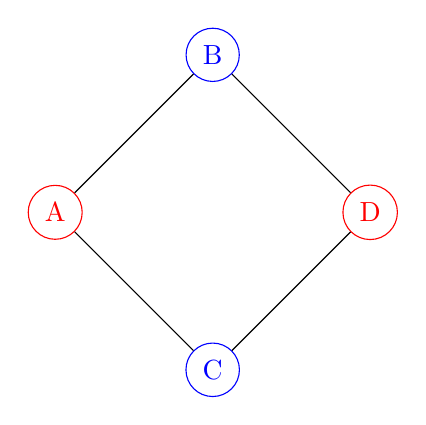
\begin{tikzpicture}%
                \node[shape=circle,draw=red,color=red] (A) at (0,2) {A};
                \node[shape=circle,draw=blue,color=blue] (B) at (2,4) {B};
                \node[shape=circle,draw=blue,color=blue] (C) at (2,0) {C};
                \node[shape=circle,draw=red,color=red] (D) at (4,2) {D};

                \path [-] (A) edge (B);
                \path [-] (A) edge (C);
                \path [-] (B) edge (D);
                \path [-] (C) edge (D);
            \end{tikzpicture}
        \end{center}\vspace*{2pt}%
    }%
    \begin{code}
        {Program}{python}
graph = {
    "A": ["B", "C"],
    "B": ["A", "D"],
    "C": ["A", "D"],
    "D": ["B", "C"],
}

color = {
    "A": 0,
    "B": 0,
    "C": 0,
    "D": 0
}

for parent, children in graph.items():
    for child in children:
        if color[child] == color[parent]:
            color[child] += 1

print(color)
print(len(set(color.values())))
    \end{code}
    \begin{code}
        {Output}{text}
{'A': 0, 'B': 1, 'C': 1, 'D': 0}
2
    \end{code}

\end{document}